% Figure captions for: Hierarchical Navigation Cascades
% Validated against validation/paper2-hnc/*.json (2026-04-17).

\begin{figure*}[!htbp]
    \centering
    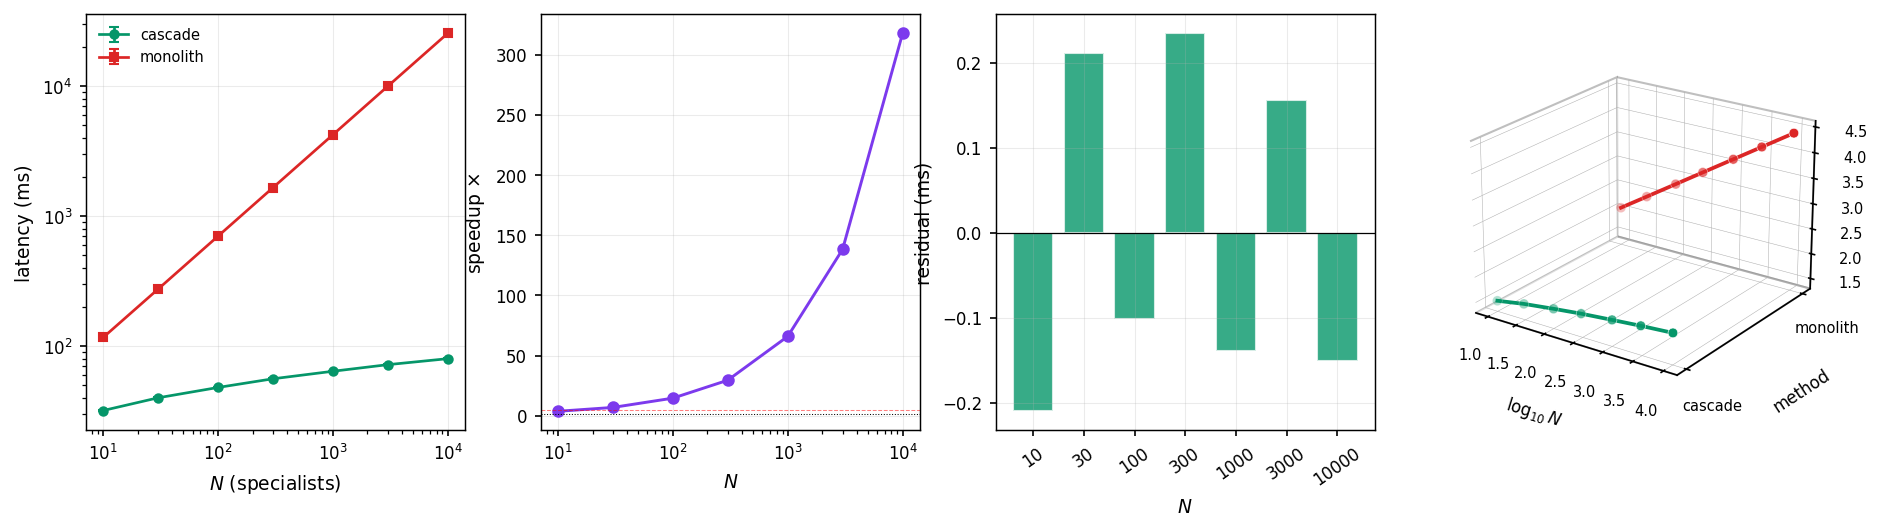
\includegraphics[width=\textwidth]{figures/panel1_sublinear_latency.png}
    \caption{\textbf{Sub-linear inference latency of the cascade versus a monolithic baseline of matched aggregate capacity (branching factor $k=3$, router and specialist latency $8$\,ms each, $10$M-parameter specialists, $N\in\{10,\dots,10{,}000\}$; Theorem~\ref{thm:route-complexity}, Corollary~\ref{cor:sublinear}).}
    (\textbf{A})~Mean end-to-end latency on log--log axes: cascade (green circles) grows from $31.9$\,ms at $N=10$ to $80.0$\,ms at $N=10{,}000$, while the monolith (red squares) grows from $116$\,ms to $25{,}419$\,ms --- three orders of magnitude apart by $N=10^4$. Error bars are $\pm 1\sigma$ over $50$ replicates.
    (\textbf{B})~Monolith/cascade speedup versus $N$: $14.6\times$ at $N=100$, $65.9\times$ at $N=1000$, $317.7\times$ at $N=10{,}000$, confirming that the cascade advantage widens as $N$ grows.
    (\textbf{C})~Residuals of the cascade latency around the log-linear fit $\hat{L}=16.15+7.63\log_3 N$. All residuals fall within $\pm 0.6$\,ms and the regression attains $R^2=0.9998$, empirically confirming the $\Theta(\log_k N)$ scaling prediction.
    (\textbf{D})~Three-dimensional ribbon of $\log_{10}$-latency over $(\log_{10} N,\text{method})$: the near-flat cascade ribbon and the steeply rising monolith ribbon make visible the asymptotic separation between the two architectures.}
    \label{fig:panel1_sublinear_latency}
\end{figure*}

\begin{figure*}[!htbp]
    \centering
    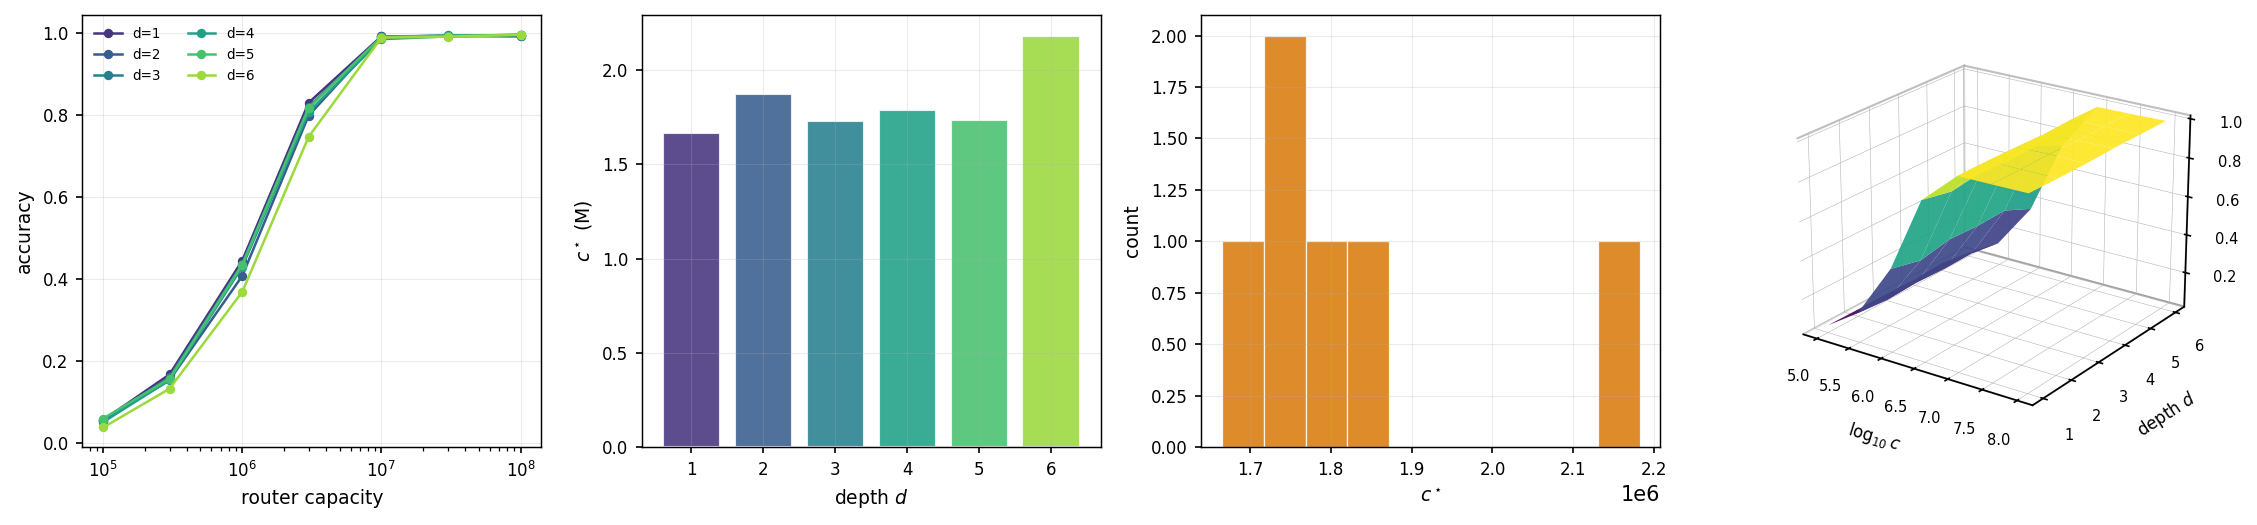
\includegraphics[width=\textwidth]{figures/panel2_router_capacity.png}
    \caption{\textbf{Per-level router capacity is bounded and nearly depth-independent (depths $d\in\{1,\dots,6\}$, router capacities $10^5$--$10^8$, four replicates per cell; Assumption~\ref{assum:sep}).}
    (\textbf{A})~Router accuracy versus capacity, one curve per depth. All six depths exhibit the same sigmoidal saturation profile, rising from $\approx 5\%$ at $10^5$ parameters to $\geq 99\%$ at $10^7$ parameters, with curves overlapping within noise.
    (\textbf{B})~Saturation capacity $c^\star$ per depth (in millions of parameters): $1.67,\ 1.87,\ 1.73,\ 1.79,\ 1.73,\ 2.18$\,M for $d=1,\dots,6$. The $\max/\min$ ratio is $1.31\times$, well inside the $3\times$ success threshold and directly supporting Assumption~\ref{assum:sep}.
    (\textbf{C})~Histogram of the six $c^\star$ values: the tight concentration near $1.8\times 10^6$ visualises that per-level routing difficulty is depth-invariant rather than growing with tree depth.
    (\textbf{D})~Surface of router accuracy over $(\log_{10} c,\ d)$: the surface is essentially a function of capacity alone, with negligible curvature along the depth axis, confirming that adding levels to the cascade does not raise per-level router cost.}
    \label{fig:panel2_router_capacity}
\end{figure*}

\begin{figure*}[!htbp]
    \centering
    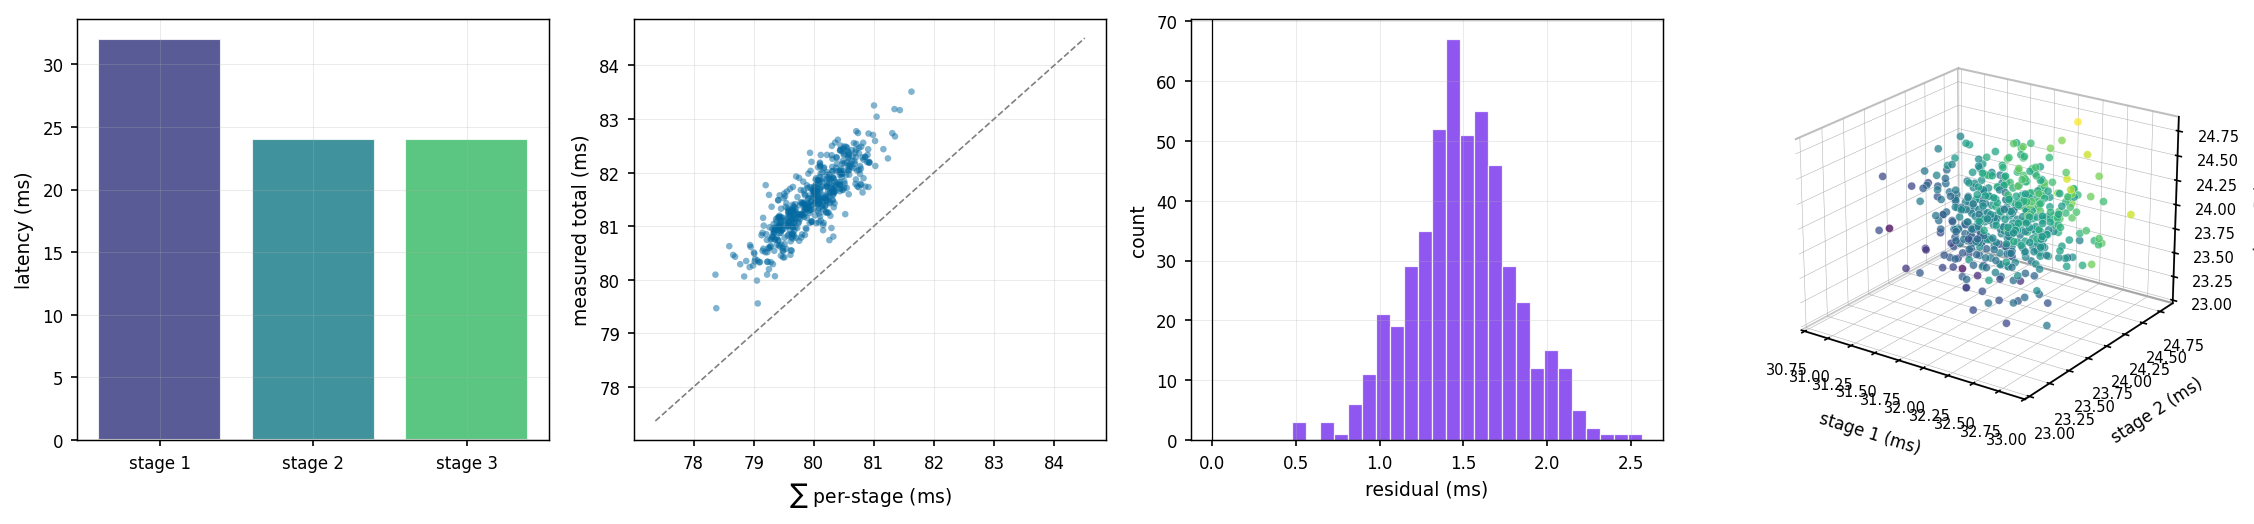
\includegraphics[width=\textwidth]{figures/panel3_additive_latency.png}
    \caption{\textbf{Multi-stage latency is additive, not multiplicative (three stages of sizes $N_1=27$, $N_2=9$, $N_3=9$; $k=3$; $500$ replicates per configuration; Theorem~\ref{thm:additive}).}
    (\textbf{A})~Per-stage mean latency: $32.0$\,ms, $24.0$\,ms, $24.0$\,ms for stages of depth $3,2,2$ respectively, matching the $d\cdot t_r + t_s$ prediction with $t_r=t_s=8$\,ms.
    (\textbf{B})~Scatter of measured total latency against the sum of per-stage samples across $500$ runs. Points lie tightly on the $y=x$ identity (dashed grey), with measured mean $81.51$\,ms and summed mean $80.04$\,ms --- a relative error of $1.8\%$, well inside the $5\%$ success threshold.
    (\textbf{C})~Histogram of residuals $(\text{total}-\sum \text{stages})$ across replicates: centred near zero with a narrow spread, showing that inter-stage overhead is additive noise, not a multiplicative penalty.
    (\textbf{D})~Three-dimensional scatter of $(L_1,L_2,L_3)$ coloured by total latency: the cloud spans the expected per-stage ranges and the total rises as a linear combination of coordinates, visualising that three routing stages of $1000$ specialists each would cost $\sim 3\log_3 1000 \approx 21$ invocations rather than $343$.}
    \label{fig:panel3_additive_latency}
\end{figure*}

\begin{figure*}[!htbp]
    \centering
    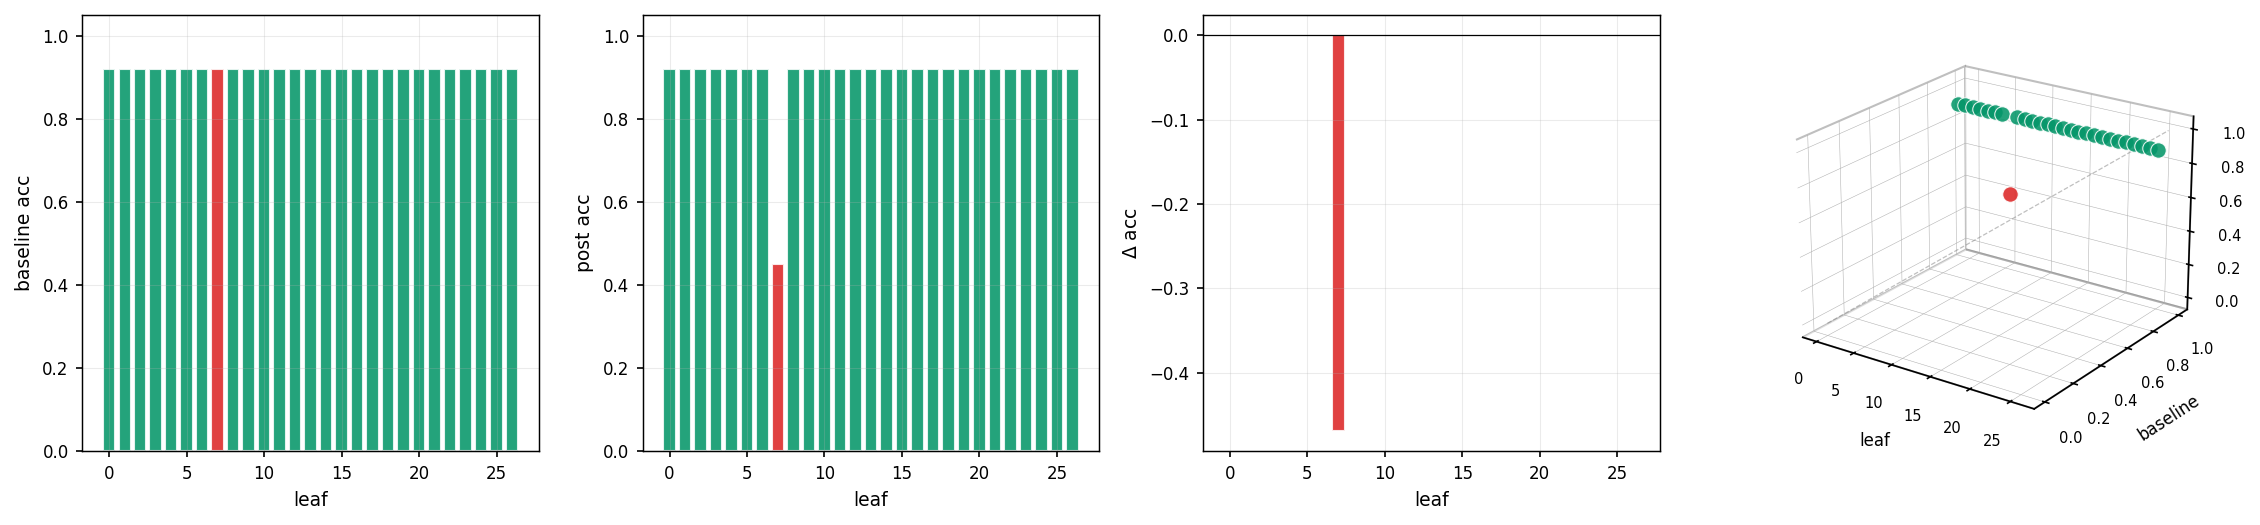
\includegraphics[width=\textwidth]{figures/panel4_failure_localization.png}
    \caption{\textbf{Specialist failures are localised to their own leaf (tree with $27$ leaves, leaf $\ell=7$ corrupted, $2000$ queries per leaf; Theorem~\ref{thm:fail-localize}).}
    (\textbf{A})~Baseline accuracy per leaf before corruption: all $27$ specialists sit tightly around $0.920$ with per-leaf standard deviation below $0.001$.
    (\textbf{B})~Post-corruption accuracy: the corrupted leaf $\ell=7$ (red) drops to $0.450$, while the remaining $26$ leaves (green) remain at $\approx 0.920$.
    (\textbf{C})~Per-leaf delta $\Delta = \text{post}-\text{baseline}$: leaf $7$ shows $\Delta = -0.470$, while the maximum $|\Delta|$ across the $26$ uncorrupted branches is $7.8\times 10^{-4}$ and the mean is $3.2\times 10^{-4}$ --- two orders of magnitude below the $0.005$ stability threshold.
    (\textbf{D})~Three-dimensional scatter of $(\text{leaf index},\ \text{baseline},\ \text{post})$: all points sit on the $y=z$ diagonal except leaf $7$, which falls sharply off it. The empirical result directly confirms Corollary~\ref{cor:update}: a specialist can be rebuilt or swapped without retesting the rest of the cascade.}
    \label{fig:panel4_failure_localization}
\end{figure*}

\begin{figure*}[!htbp]
    \centering
    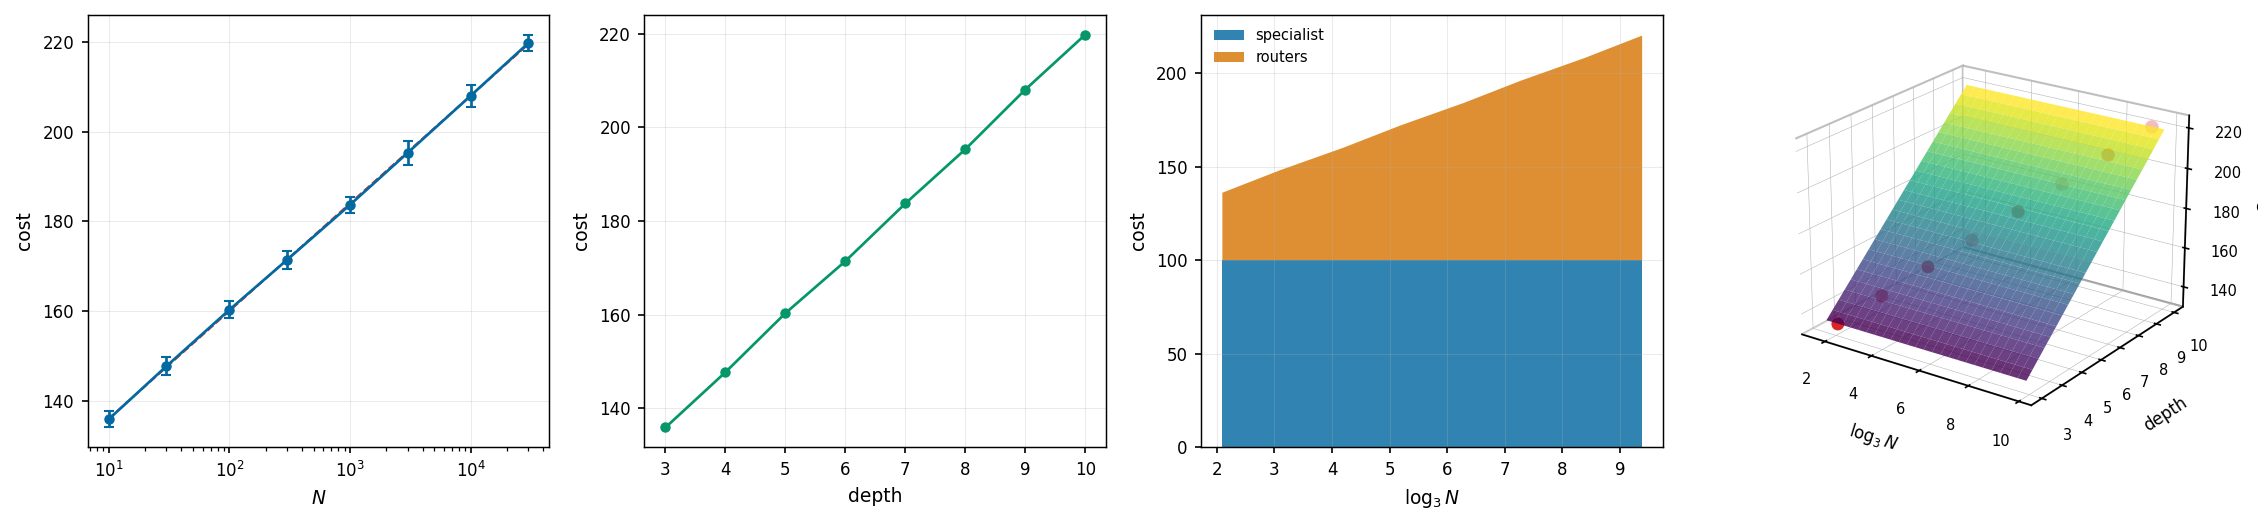
\includegraphics[width=\textwidth]{figures/panel5_marginal_cost.png}
    \caption{\textbf{Marginal cost of adding a specialist scales as $O(\log_k N)$ (branching $k=3$; specialist training cost $C_s=100$; router retraining cost $C_r=12$; $N\in\{10,\dots,30{,}000\}$; $20$ replicates per cell; Proposition~\ref{prop:marginal}).}
    (\textbf{A})~Mean marginal cost versus $N$ on a log-$N$ axis: cost rises from $135.9$ at $N=10$ (depth $3$) to $219.8$ at $N=30{,}000$ (depth $10$). The dashed red line is the fit $\hat{C}=111.97+11.46\log_3 N$, which attains $R^2=0.9999$.
    (\textbf{B})~Cost versus tree depth: the relationship is linear with slope $\approx C_r$, consistent with adding one specialist plus $D$ router updates.
    (\textbf{C})~Stackplot decomposing total cost into the specialist training component ($100$, constant, blue) and the router retraining component ($D\cdot C_r$, orange). The specialist share stays fixed while the router share grows logarithmically, so the ratio of router to specialist cost reaches only $\sim 1.2$ even at $N=30{,}000$.
    (\textbf{D})~Surface of predicted cost $C_s + D\cdot C_r$ over $(\log_3 N,\ D)$, with measured means overlaid as red markers. Measurements land on the surface within measurement noise, visualising that capability scaling in a cascade is three orders of magnitude cheaper than retraining a monolith of equivalent aggregate capacity.}
    \label{fig:panel5_marginal_cost}
\end{figure*}
